\part{Application}
\chapter{Inertial Waves in a Rotating Cone}

\section{Introduction}

Following the introduction and validation of the immersed boundary methods
we now want to exemplarly investigate a fluid system using these methods
and find out if we can reproduce some of the expected physical properties.
In relation to the research focus of the geophysical fluid mechanics research group, there are a variety
topics of interest.
One area of research lies in the exploration of dynamo effects in geological and stellar system.
In particular this means the generation of magnetic fields by electrically conducting fluids on large scales.
In this thesis we will not consider MHD-equations.
However in general it is considered that the helicity of a fluid domain $\Omega$, given by

\begin{align}
    \int_{\Omega}\dif V  \vec{u} \left( \nabla \times \vec{u} \right)
\end{align}

is directly linked to dynamo action \citep{moffat1978}.
Therefore it would be interesting to find a system which exhibits a large helicity,
as a possible candidate for future researches of the geo dynamo.
Furthermore we are interested in the propagation of inertial waves in different fluid domains.
In particular we want to examine the ability to generate inertial modes or wave attractors
for the geometry we will introduce in this chapter.
%For the system we describe in the following section one further application
%would be to study inertial wave excitaton by turbulence. (MORE DETAIL THIS AND ALPHA FUNCTION)
-introduction cone here?
-lineariztaino etc 2d but 3d wegen turbulence
The objective we have in mind is the numerical computation of inertial wave excitation inside a librating cone.

\section{Inertial Waves in a Librating Cone}
\label{cone:theorie_exp}

\subsection{Theoretical Description}

We beginn with a short theoretical description of the problem adapted from \citep{Greenspan1969}, \citep{Beardsley1970}.
For the cone we make the comparsion to the two-dimensional case of a wedge.
This system is based on the idea to introduce a geometric shape, containing a singularity.
Here we want to discuss the propagation of an inertial wave emitting at one of the upper edges of
the wedge as shown in figure \ref{cone:theorie}.
Here we consider an inviscous fluid.
For each reflection the propagation angle with respect to the rotation axis stays constant.
Let us recall from  section \ref{theorie:sec:iwreflec}, that
for $\theta<\alpha$ we have a subcritical reflection,
thus a downward traveling wave ray is reflected downslope.

\begin{figure}[!tp]
  \begin{minipage}[c]{0.6\textwidth}
      \centering
        \resizebox{0.7\textwidth}{!}{
       \import{gfx/cone//}{cone.pdf_tex}
      }
  \end{minipage}
  \begin{minipage}[c]{0.3\textwidth}
      \caption{
          Propagation of an inertial wave emitted from the top edge of a wedge,
           where $\Theta$ indicates the direction parallel to the group velocity
            $\vec{c_g}$, s $L$ and $L^{\prime}$ are the path lengths before and after a reflection.
      \label{cone:theorie}
      }
  \end{minipage}
\end{figure}

As a results the wave ray travels towards the lower vertex of the wegde.
It can be shown from the reflection properties given by equation () and (),
that the time for a wave ray to travel the path between two reflections is constant \citep{Beardsley1970},
which is

\begin{align}
    \frac{L}{|\vec{c}_g|} = \frac{L^{\prime}}{|\vec{c^{\prime}}_g|}
\end{align}

This means that the overall propagation time into the apex of the cone becomes infinity, along with the energy density and the wave number.
In conclusion it follows that since no reflection out of the cone apex can occur, the possibilty of inertial modes is not given.\\

\subsection{Experiment}

In order to test these theoretical assumptions  an experimental study was performed by \citep{Beardsley1970}.
The schematic setup of the experiment is shown in figure \ref{cone:setup_experiment}.\\
In the first part of the experiment a plexiglass cylinder, containing a conical shaped cavity,
of height $H=\SI{19.95}{\centi\meter}$ and a radius of $r=\SI{19.95}{\centi\meter}$ was used.
The apex half angle was set to $\alpha=24^{\circ}3.7^{\prime}$ degree.
For the rotation rate a frequency of $\omega =\SI{6.28}{\radian\per\second}$ was chosen.
As a fluid, water was used, the resulting viscosity, given by \citep{tipler2003}, is $\nu = \SI{1.0}{\milli\pascal\second}$.
The resulting Ekman number is

\begin{align}
    \Ekman = \frac{\nu}{\omega r H^2} \approx 7.72\cdot 10^{-6}
\end{align}

In order to exite inertial waves the cone is librating.
The total rotation rate is given by

\begin{align}
\Omega(t) = \Omega_0 + \epsilon \omega \cos(\omega t)
\end{align}

where $\omega$ is the libration frequency.
This means that excitation mechanism results from wall friction, induced
by a modulation of the constant rotation frequency $\Omega_0$.

\begin{figure}[!bt]
      \centering
        \resizebox{0.6\textwidth}{!}{
       \import{gfx/cone///}{experiment.pdf_tex}
      }
      \caption{
      experiment
      \label{cone:setup_experiment}
      }
\end{figure}

For the analysis the dynamic pressure field was measured at at different depths along the rotation axis,
with the libration frequency in the range of $0.25\leq\omega/2\Omega\leq2$.
The pressure and phase lag spectrum, for each measurement height, show that for this setup
no inertial modes can be observed.\\
In the second part of the experiment the apex of the cone was replaced by a frustum through the
insertion of a bottom plate in the cone, at the position $z/H = 0.261$.
With this setup yields the possibility that a wave ray can be reflected on bottom of frustum.
The pressure and phase lag spectrum in this setup show that
independent of the height resonances occur which can be associated with standing waves.
Hence inertial modes exist.

\section{Numerical Implementation of Libration}

For the numerical implementation of the experiment, we will use a modified set of the equations
introduced in section \ref{THEORIE:ROT}.
We have to concern that the system has now a time-depent rotation rate.
For the non-dimensional system, with $\vec{u}^* =  \vec{u} (|\vec{\Omega}|L)^{-1}$, we set

\begin{align}
    \vec{\Omega(t)} = 1 \; + \; \epsilon \cos(\omega t)\vec{e}_z
\end{align}

There are two options, which should be considered here.
First of all, we can choose a rotating coordinate system with a constant velocity $\Omega_0$.
This means the we can directly use the equations () to (). Since the overall rotation rate of the system is
modulated, it is necessary to introduce the boundary conditions

\begin{align}
    \vec{v}|_{Border}  = \Omega \times \vec{r} = \begin{pmatrix}
           -y \epsilon \cos(\omega t) \\
           x \epsilon \cos(\omega t) \\
           0\\
         \end{pmatrix}
\end{align}

However, obtaining a linearized version of the boundary methods is not as easy.
In addition we think it is safer to use No-Slip boundaries with zero velocity, as
the taylor-couette system showed that other boundarie velocities can create a larger numerical error.
The alternative option is the introduction of an accelerated frame of reference.
In this case the boundary conditions do not need to be modified, but the coriolis forcing term is given by \citep{Tilgner2007}.

\begin{align}
    \vec{f} &= 2 \vec{\Omega} \times \vec{v} + \pdn[]{t}\left(\vec{\Omega} \times \vec{v} \right)
            = \begin{pmatrix}
           -y \omega \epsilon \cos(\omega t) \\
           -x \omega \epsilon \cos(\omega t) \\
           0\\
         \end{pmatrix}
            + 2\begin{pmatrix}
           - ( 1 + \epsilon \sin(\omega t)v_x \\
             ( 1 + \epsilon \sin(\omega t)v_y \\
           0\\
         \end{pmatrix}
            = \begin{pmatrix}
           -y \epsilon \cos(\omega t) \\
           -x \epsilon \cos(\omega t) \\
           0\\
         \end{pmatrix}
\end{align}

In the last step the linearization was introduced.
Finally the non-linear advection term was removed from the equations of motion, which
are then given by

\begin{align}
    \label{theorie:rotns}
    \pdn[u]{t} = -c^2\nabla \rho + \Ekman \Delta \vec{u} + \vec{f} \qquad;& \qquad  \nabla \vec{v} = 0
\end{align}

Finally one additional stability criterion shall be introduced,
It is important that the time for propagting information from on side of the domain
to the other, is much smaller than the overall rotation rate.
\footnote{Private communication with A. Tilgner}
Since information inside the fluid domain propagates at an artificial sound speed,
this yields the estimation

\begin{align}
    t = \sqrt{\frac{2}{c^2}} << 2\pi
\end{align}

A good estimation is given by setting $c^2 = 500$.
It could be observed that otherwise, not only physical wrong results are obtained but also
numerical instabilitys can occur.
\footnote{Private communication with O. Goepfert}
\newpage

\subsection{Setup}

This section introduces the setup which has been used for the simulations presented in this chapter.
Figure \ref{cone:setup_image} shows the geometry of the fluid domain. The parameters are given by

\begin{multicols}{2}
\begin{description}
    \item[$H$]{Total height of the simulation domain}
    \item[$h_c$]{Height of the Cone}
    \item[$h_t$]{Height of the bottom plate for a frustum}
    \item[$r$]{Radius of the bottom plate}
    \item[$O$]{Offset at the top of the Cone}
    \item[$\alpha$]{Slope of the Cone}
    \item[$\Omega$]{Rotation rate}
    \item[$\omega$]{Frequency of the libration}
\end{description}
\end{multicols}

This convention will be used throughout rest of this chapter.
For the implementation the testcase function template introduced in chapter () is used.
The use of the different parameters with this template is shown in Appendix ().

\begin{figure}[!bp]
  \centering
        \resizebox{0.6\textwidth}{!}{
       \import{gfx/cone/conesim//}{setup.pdf_tex}
      }
      \caption{Numerical Setup for the Simulations \label{cone:setup_image} }
\end{figure}
\clearpage

\section{Simulation of a Librating Cylinder}
\label{cone:sec:lib_cylinder}

As a first step towards the implemenation of the librating cone,
simulations of fluid flow in a librating cylinder were carried out.
Despite the the theoretical and experimental results, discussed in section \ref{cone:theorie_exp},
it is diffult to find results in literature which would be suitable for an appropiate validation.
For the cylinder on the other hand, theoretical and numerical results are available.
A theoretical solution can be found in \citep{Greenspan1990}, and shall be summarized here.
For the inviscid case the problem can be reduced to a Poincar\'{e} equation for the pressure,
which is solved in cylindrical coordinates by

\begin{align}
    p_{nmk}(r, \theta, z ) = J_{|k|}\left(\frac{\xi_{nmk}r}{a} \right)\cos(n\pi)\exp(ik\theta)
\end{align}

where $a=\nicefrac{r}{H}$ is the aspect ration of the cylinder, $n\in\mathbb{Z}$

where $\xi$ denotes the radial wavenumber,

\begin{align}
    \xi \frac{\dif}{\dif \xi}J_{|k|}(\xi) + k \sqrt{1 + \frac{\xi^2}{n^2\pi^2a^2}} \; J_{|k|}\left(\xi\right) = 0
\end{align}

The eigenvalue of the solution
\begin{align}
    \lambda_{nmk} = 2\sqrt{1 \; + \;\frac{ \xi_{nmk}^2}{n^2\pi^2a^2}}
\end{align}


-theoretically greenspan  blabla

The velocity of a mode is given by in cylindr. coord


-mode kann dann festgelegt werden durch tuple bla.\\
The numerical setup is  given by ..
-Nx  = 128 ,lx, ly
-aspect ration
-ekman number
-further condition timestep
-omega in bla
\newpage

\subsection{Results \& Discussion}




\begin{align}
    \left<v_z^2 \right>(t) =  \int \dif V v_z(t)^2 \approx \sum_{i, j, k}^{N_x,N_y,N_z} \Delta x \Delta y \Delta z \left.v_z(t)^2 \right|_{i,j,k}
\end{align}

\begin{align}
    A\left(\left<v_z^2\right>\right) = \frac{\max(\argmax(\left<v_z^2\right>_{v})) - \max(\argmin(\left<v_z^2\right>_{v}))}{2}
\end{align}

-bilder
-description


\begin{figure}[!pt]
  \centering
  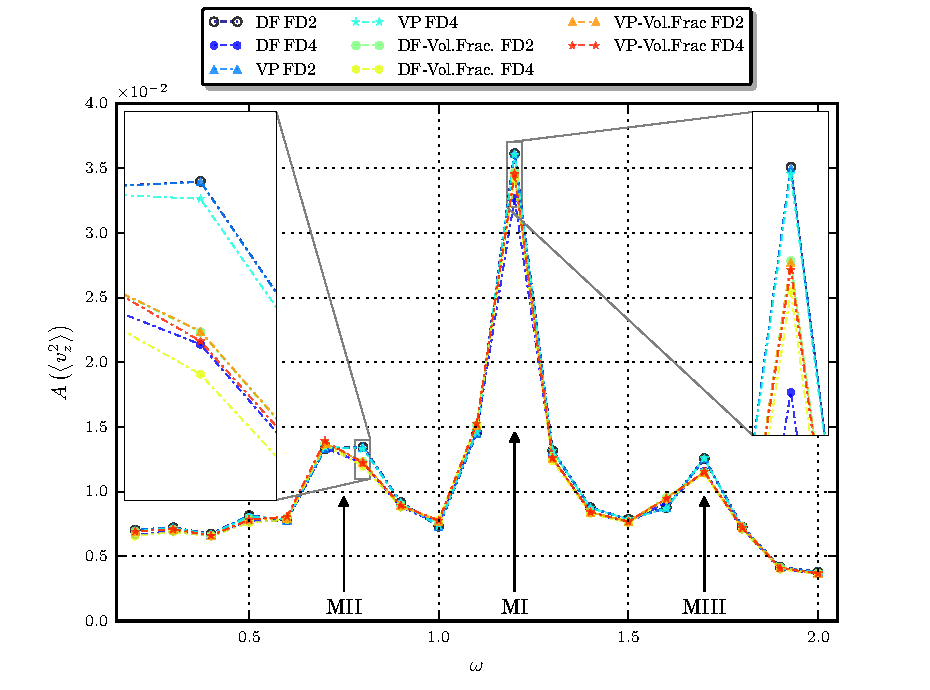
\includegraphics{gfx/cone/cylinder/cylinder.pdf}\label{fig:cone:cyl}
  \caption{blabla}

  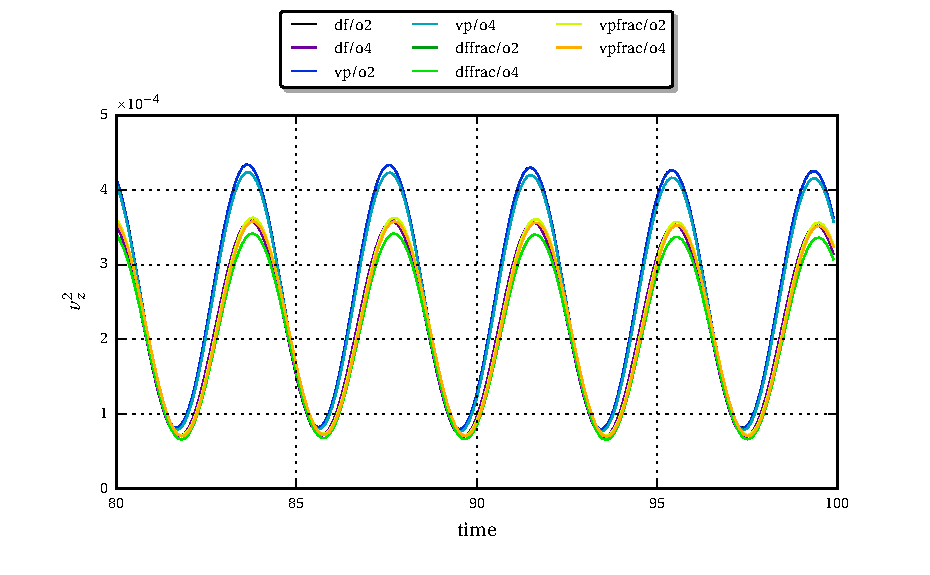
\includegraphics{gfx/cone/cylinder/cyl_vz.pdf}\label{fig:cone:cyl_time}
  \caption{blabla}
\end{figure}
\newpage

-behaviour known theorie
- paper kurz erklären symetrie warum fehlen bestimmte moden ? ?

As a first system we want to investigate the

- erstes test system cylinnder\\
- expectation

- verglein von den bedien implementierungen\\
- first test omega = 1.2 ...\\
- diskussion rand compare to tcflow \\
- test serie verschiede methoden\\
- spektrum dargesstel\\
- evtl raytracer  comparison
- heliziätte dargstellt\\
- results diskussion ip kaputt heli 0 etc \\
\subsection{Numerical Viscosity}

\newpage

\section{Simulation of a Librating Cone}

In this section we will discuss the different numerical simulations, which has been performed
with a librating cone. We begin with the comparison to the experiment performed by \citep{Beardsley1970}.
As a next step we analyse the physical behaviour when performing the transition from a cylinder
to a cone and finally  we will investigate the influence of different offsets on top of the cone.
All simulations performed in this section use the introduced setup with different geometric parameters.
As a IBM we choose the direct forcing  method of second order.

-as a convention we refer to frustom cone etc

\subsection{Simulation of the Experiment}

The setup for this simulation is oriented on the experimental setup given by \citep{Beardsley1970}, which
we disussed in section ().
In the first part of the experiment a plexiglass cylinder of height $H=\SI{19.95}{\centi\meter}$ and a radius of
$r=\SI{19.95}{\centi\meter}$ was used. The apex half angle was set to $24^{\circ}3.7^{\prime}$ degree,
which relates to our setup with $\alpha=65^{\circ}56.3^{\prime}$
For the rotation rate a frequency of $\omega =\SI{6.28}{\radian\per\second}$ was chosen.
As a fluid, water was used, the resulting viscosity,given by \citep{tipler2003}, is $\nu = \SI{1.0}{\milli\pascal\second}$.
The resulting Ekman number is given by

\begin{align}
    \Ekman = \frac{\nu}{\omega r H^2} \approx 7.72\cdot 10^{-6}
\end{align}

In the second part of the experiment the apex of the cone was replaced by a frustum through the
insertion of a bottom plate at the position $z/H = 0.261$.
For the simulation we choose an Ekman number of $\Ekman =  10^{-4}$, since a simulation of higher ekman numbers is
diffcult to realise due to the computational effort.
Furthermore we set $\alpha = \arccos(1/2) = 60^{\circ}$, $H=1$ and $r=0.5$.\\
This means that for $\omega=1$, the propagation of an inertial wave package is parallel to the slope of the cone.
For the offset on top of the cone, we obtain the condition

\begin{align}
    o = H - h_c =  1 - r\tan{\alpha} \approx 0.134
\end{align}

The simulation has two setups in analogy to the experiment.For the second part the bottom plate is set to $h_b=0.25$.
A series of simulations of these systems where performed, with the parameters

\begin{center}
\vspace*{0.7ex}
\begin{tabular}{c|c|c|c|c|c|c }
%\begin{tabular}{p{0.1\linewidth}| p{0.1\linewidth}| p{0.1\linewidth}|  p{0.1\linewidth}| p{0.1\linewidth}| p{0.1\linewidth} }
$ \leftarrow  \omega \rightarrow $ & $\Delta t$ & $\Delta x$ & $c^2$ & \Ekman  & $l_x, l_y, l_z$ & $T_{end}$\\
\hline
$[0.2,\; 2], \Delta w = \nicefrac{1}{10}$ & $10^{-5}$ & $\nicefrac{1}{128}$ & 500 & $10^{-4}$  & (\{1, 0.75\}, 1, 1) & 100\\
\end{tabular}
\vspace*{0.7ex}
\end{center}

\clearpage
%\begin{figure}[!tp]
%  \begin{minipage}[c]{0.6\textwidth}
%      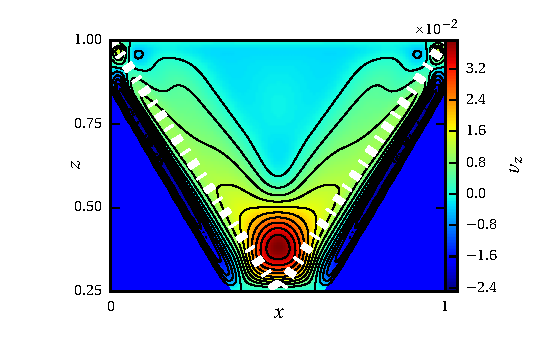
\includegraphics{gfx/cone/experiment/contour.pdf}\label{fig:mask_vp}
%  \end{minipage}\hfill
%  \begin{minipage}[c]{0.3\textwidth}
%  \caption{Stability regions for $\Omega_s$ for different Runge-Kutta methodsi
%    Stability regions for $\Omega_s$ for different Runge-Kutta methodsi
%  }
%  \label{fig:num_rkstab}
%  \end{minipage}
%\end{figure}
%
%\begin{figure}[!tp]
%  \begin{minipage}[c]{0.3\textwidth}
%  \caption{Stability regions for $\Omega_s$ for different Runge-Kutta methods
%  Stability regions for $\Omega_s$ for different Runge-Kutta methodsi
%  }
%  \label{fig:num_rkstab}
%  \end{minipage}
%  \hfill
%  \begin{minipage}[c]{0.6\textwidth}
%      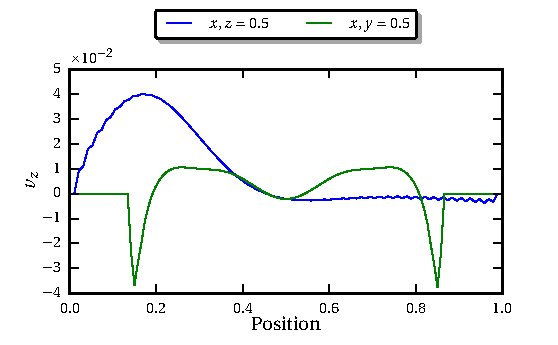
\includegraphics{gfx/cone/experiment/error.pdf}\label{fig:mask_vp}
%  \end{minipage}
%\end{figure}

\begin{figure}[!bp]
  \centering
  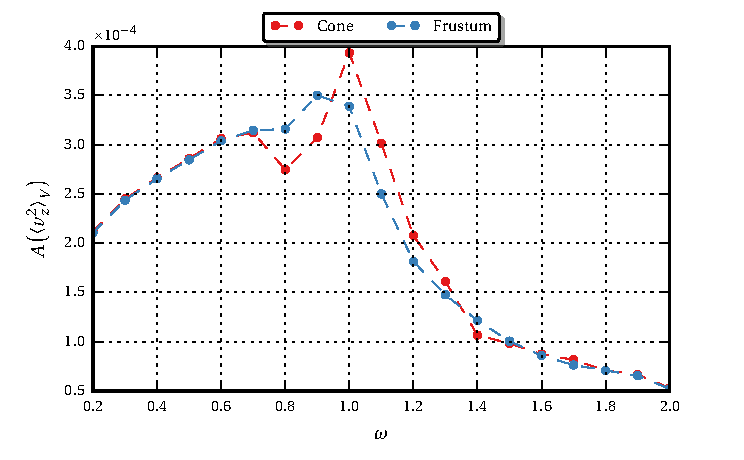
\includegraphics{gfx/cone/experiment/experiment.pdf}
  \caption{Amplitude $A\left(\left<v^2_z\right>_V\right)$ as a function of the libration frequency $\omega$,
            for a cone and a frustum.  \label{fig:cone_expseries} }
\end{figure}

\subsubsection{Results \& Discussion}
\label{cone:exp}

The results of the simulations are shown in figure \ref{fig:cone_expseries}.
For both cases, the frustum and the cone, we can observe an increase in $A\left(\left<v^2_z\right>_V\right)$
from $\approx 2\cdot10^{-4}$ at $\omega=0$ to  $\approx 3.4\cdot10^{-4}$ for the frustum and $\approx 4\cdot10^{-4}$ for the cone,  at $\omega=1$.
From here one the Amplitude decreases to $\approx 5\cdot10^{-5}$ at $\omega=2$.\\
A difference between the two setups can be observed in the surrounding area of $\omega=1$.
For the cone the increase of the amplitude is interrupted at $\omega=0.6$, a minimum can be observed at $\omega=0.8$, followed by
a peak at $\omega=1$. For the frustum the minium is not directly visible but it can be noted that the
amplitude does not increase as much at $\omega=0.7$, as for lower frequencies.\\
The maximum occurs at $\omega=0.9$, in comparison to the cone we see an increase in the amplitude of $\approx 5\cdot10^{-5}$.
However, it has to be considered, that due do the stepwidth of $\Delta \omega = 0.1$, the exact position of the maxima is
not apparent.\\
One possible assumption, regarding the position of the maximum with respect to the frequency, is that
the expansion of the frustum with a tip  results in a shift to lower frequencies.
The left shift in the decrease for $\omega > 1$ furthermore supports this idea.\\
Overall it appears that the spectrum can be divided into two domains $\Omega_1~=~\{0\leq\omega<1$\} and $\Omega_2~=~\{1\leq\omega\leq2\}$.
This result is not unexpected, since we choose the slope $\alpha$ of the cone such that for $\omega=1$, it is parallel
do the group velocity $\vec{c}_{g}$.
For $\omega\in\Omega_1$ the results for both setups are similar, since in this domain, the cone tip does not act as an attractor.
An inertial wave propagates the top, after a reflection on the side of the cone.
Hence, for both setups we obtain a similar spectrum.
The differences occur when $\omega$ is reaching the critical slope, in this scenario an inertial wave propating from the
top edges, travereses directly into the apex of the cone, or is reflected slightly at he bottom plate of the frustum.
As a results we see the increase in the amplitude.
For $\omega\in \Omega_2$ we would expect further reflections for the frustum, however the similar
decay of the amplitude refutes this assumption.\\
The results of the simulation do not match with the ones of the experiment we discussed in section ().
A possible explanation we want to propose here, is the use of a different Ekman number, which is of order $10^{-4}$ in contrast
to the one of the experiment of $10^{-5}$.
As a consequence the width of an inertial wave packet, given by $\propto \Ekman^{1/3} \approx 2\cdot10^{-2}$ (see \citep{} or section...),
is around twice the size as in the experiment. We assume that as a results a wave reflecting on the bottom of the frustum
is strongly damped due to wall friction.
DISCUSS T:\\
damping  could be propt $\Ekman \vec{K}$.

\subsection{Transition to from a Cylinder to a Cone}

We now want to further investigate the results from the previous simulation.
The assumption was made, that the inserted bottom plate is to narrow to support an efficient reflection
of inertial waves, due to frictional losses at the bottom of the cone. Thus, the next objective would be to
test the influence of different gap radii $r$.\\
We propose a setting where we begin with the possible largest bottom gap, which is $r=0.5$.
As a next step we iteratively decrease the size of the gap by $\Delta r = 0.125$ until $r=0$ is reached.
An alternative approach to this woudld be to change the offset from the bottom of the cone, which would result in a constant
slope but different heights of the simulation domain.
The influence on the simulation domain is shown in figure ()(b).
For $r=0.5$ the domain is given by a cylinder, which than transforms into a cone with a frustum and finally with an apex for $r=0$.
The main simulation parameters are given by

\begin{center}
\vspace*{0.7ex}
\begin{tabular}{c|c|c|c|c|c|c|c }
%\begin{tabular}{p{0.1\linewidth}| p{0.1\linewidth}| p{0.1\linewidth}|  p{0.1\linewidth}| p{0.1\linewidth}| p{0.1\linewidth} }
$\leftarrow r \rightarrow$ & $ \leftarrow  \omega \rightarrow $ & $\Delta t$ & $\Delta x$ & $c^2$ & \Ekman  & $l_x, l_y, l_z$ & $T_{end}$\\
\hline
$[0,\; 0.5], \Delta r =0.125$ & $[0.2,\; 2], \Delta w = \nicefrac{1}{10}$ & $10^{-5}$ & $\nicefrac{1}{128}$ & 500 & $10^{-4}$  & (1, 1, 1) & 100\\
\end{tabular}
\vspace*{0.7ex}
\end{center}
%
%\subsubsection{Results \& Discussion}
%\begin{figure}[!bp]
%      \begin{minipage}[c]{0.4\textwidth}
%      \centering
%        \resizebox{0.8\textwidth}{!}{
%       \import{gfx/cone/transition//}{attractor.pdf_tex}
%      }
%      \end{minipage}\hfill
%  \begin{minipage}[c]{0.6\textwidth}
%      \caption{
%          Wave attractor in a cylinder $\left(\text{\colorbox{green}{\textcolor{green}{o}}{\null}}\right)$
%          and shifted\\ attractor $\left(\text{\colorbox{red}{\textcolor{red}{o}}{\null}}\right)$
%          for $r<0.5$. To maintain the same attractor the point of reflection has to be at the same height $h_r$.
%      }
%      \label{cone:theorie}
%      \end{minipage}\hfill
%\end{figure}



\subsubsection{Results \& Discussion}

The results of the simulations are shown in figure \ref{fig:cone:transition}.
For $r=0$ we can see the inertial modes of a librating cylinder, which is in accordance
to the results we discussed in section \ref{cone:sec:lib_cylinder}.
With an decrease of the radius we can observe a change in the position and amplitude of the
inertial modes. We want to exemplarly discuss this pattern for the (2, 2) mode at $\omega=1.3$, where it is the best visible.
For all other modes the transition results in a similar behvavior.\\

\begin{figure}[!pt]
  \centering
  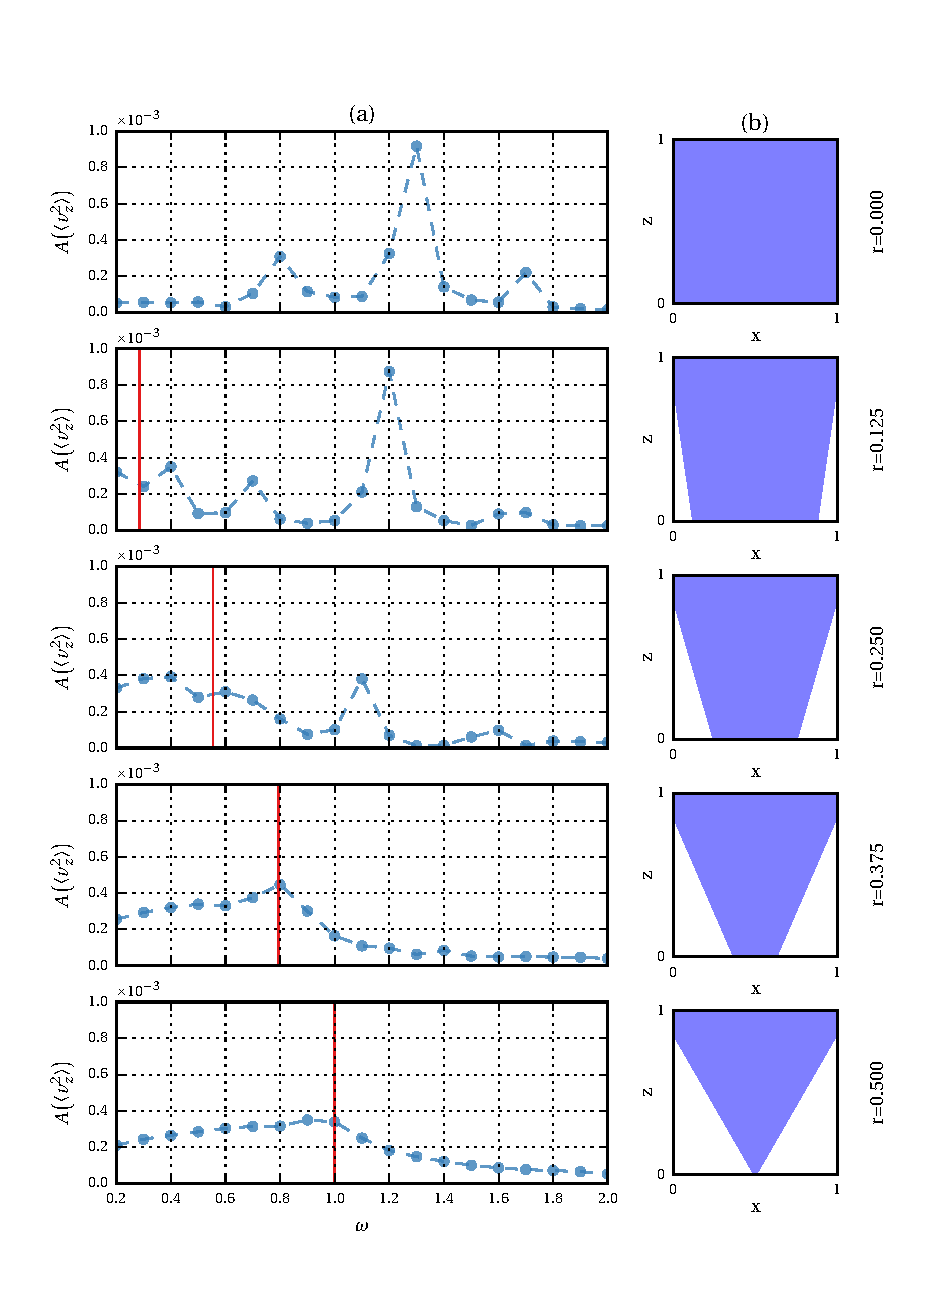
\includegraphics{gfx/cone/transition/transition.pdf}
  \caption{\label{fig:cone:transition}
    Simulation of
  }
\end{figure}

The decrease of the radius leads to a shift to lower frequencies of the (2, 2) mode,
from $r=0$ to $r=0.375$ it is of the order $\Delta \omega=0.1$.
Furthermore we can see, that during the transition a damping of the mode occurs.
For $r=0.5$ the amplitude is of order $\approx8.9\cdot10^{-3}$, for $r=0.375$ it is
$\approx8.9\cdot10^{-3}$ and for $r=0.25$ we obtain $\approx3.8\cdot10^{-3}$.\\
Whereas the first decrease of the radius does not significantly affect the amplitude,
the second decrease leads to a strong damping to less than half of the original size.
With a further decrease in $r$, the (2, 2) mode is annihilated.
\footnote{ for the possible (1, 2) mode we still can observe a slight increase of the amplitude at $r=1.4$}
One possible explanation for the shift can be given
by having a look at the inertial mode structure, for different radii as shown in figure \ref{fig:cone:phase}.\\
For $r=0.5$ we have an inertial mode, which is symmetric to the plane $h/2$.
In this plane, the waves excited from the bottom and top of the cylinder, annihilate each other and form a wave node.
An decrease of radius breaks the axial symetrie of the inertial mode.
As a result only a distorted version of the mode can exist, where the center of the wave node
is given by the intersection of the diagonals from the top to the bottom edges of the frustum.
In order to obtain the new shape it is necessary to increase the propagation angle $\Theta$,
which is equivalent to lowering the libration frequency.
We can furthermore say that for $r \rightarrow 0$, the center given by

\begin{align}
c  = r \frac{h}{r+\nicefrac{l_x}{2}}
\end{align}

converges against zero, hence a mode cannot exist in this state.
Beside the changes of the inertial modes it can be noted, that simultaneously to the decrease of the radius,
a lift of the amplitudes at lower frequencies occurs.
The vertical lines in figure \ref{fig:cone:transition} are set to the position $\omega=\Theta$.
The area $\omega<\Theta$ can again be associated with the frequency domain, where the wave propagation angle $\Theta$ is larger than
the  slope of the cone $\alpha$ and waves propgate to the top, up on reflection on the slope.
For $r=0$ we have the indentical setup to the simulation in section \ref{cone:exp}.

\begin{figure}[!pt]
  \centering
  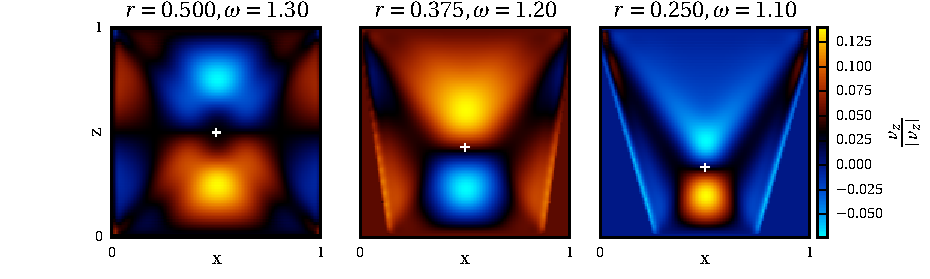
\includegraphics{gfx/cone/transition/phase.pdf}
  \caption{\label{fig:cone:phase}
    Simulation of
  }
\end{figure}

\clearpage

\subsection{Librating Cone with different Offsets at the Top}

Finally we want to improve the setup we introduced in section \ref{exp},
by considering the insights we gained from the previous simulations.
As we pointed out, the radius at the bottom of the frustum has a strong influence on
the reflection of inertial waves, due to the larger Ekman number we use in comparsion to the experiment.
Hence, we insert the bottom plate in the cone at a height of $h_b=0.375$, the resulting radius is
$r \approx 0.22$. The total height is than given by $h=0.625$,
and the slope is unchanged.
Secondly we want to adress the influence of the offset on top of the cone,
which has been left out from any discussion so far.
We assume that this offset has an strong influence for the intervall $\Theta<\alpha$,
where wave reflection to the top occurs.
In the case where $o=0$, the corners of the cone would act as an attractor, as pointed out in figure \ref{cone:img_finalattractor}.

\begin{figure}[!bp]
      \centering
        \resizebox{0.7\textwidth}{!}{
       \import{gfx/cone//}{comparison.pdf_tex}
      }
      \caption{
          Wave reflection for $o>0$ in the upper edges of the cone (left) and
          an attractor for $o=0$ (right), in the upper edges of the cone.
      \label{cone:img_finalattractor}
      }
\end{figure}

For small gap sizes it also applies that a inertial wave will be damped.
Therefore, in this simulation we will add an additional offset to the default of $\tan(\pi/3)/2$
varying in the range of $h_+ = [0, 1]$ with a stepsize of $\Delta h_+ = \nicefrac{1}{5}$.
The main simulation parameters are given by

\begin{center}
\vspace*{0.7ex}
\begin{tabular}{c|c|c|c|c|c|c|c }
%\begin{tabular}{p{0.1\linewidth}| p{0.1\linewidth}| p{0.1\linewidth}|  p{0.1\linewidth}| p{0.1\linewidth}| p{0.1\linewidth} }
$\leftarrow r \rightarrow$ & $ \leftarrow  \omega \rightarrow $ & $\Delta t$ & $\Delta x$ & $c^2$ & \Ekman  & $l_x, l_y, l_z$ & $T_{end}$\\
\hline
$[0,\; 0.5], \Delta r =0.125$ & $[0.2,\; 2], \Delta w = \nicefrac{1}{10}$ & $10^{-5}$ & $\nicefrac{1}{128}$ & 500 & $10^{-4}$  & (1, 1, 1) & 100\\
\end{tabular}
\vspace*{0.7ex}
\end{center}

Furthermore we will compute the normalized helicity of the system given by

\begin{align}
H(t) = \frac{\int_V \dif V \vec{v} (\nabla \times \vec{v})}{\int_V \dif V |\vec{v}||\nabla \times \vec{v}|}
 = \frac{\sum_{i,j,k=0}^{N_x, N_y, N_z} \vec{v}_{i,j,k} (\nabla \times \vec{v}_{i, j, k})}
 {\sum_{i,j,k=0}^{N_x, N_y, N_z}|\vec{v}_{i,j,k}|| \nabla \times \vec{v}_{i, j, k}|}
\end{align}

in the accelerated frame of reference and also for the inertial system with an additional offset in the velocity
given by $\vec{u} = \vec{u}|_{\text{rot.}} + \Omega(t) \times \vec{r}$.
\\


The discretization of the rotation operator is using a central difference of second order.
As a next step we want to furthermore analyze the decay of inertial waves for the different offsets.
For this reason we use the end state from the previous simulations and set
the libration amplitude to zero.
Furthermore we change the end time of the previous simulations by

\begin{align}
    T = \frac{1}{\Delta t} \text{floor}\left(\text{T}_{\text{end}}\frac{\omega}{2\pi}\right)\frac{2\pi}{\omega} + \frac{2\pi}{\omega}
\end{align}

to make sure that for all frequencies the librating force drops out when crossing zero.
The main simulation parameters are given by

\begin{center}
\vspace*{0.7ex}
\begin{tabular}{c|c|c|c|c|c|c|c }
%\begin{tabular}{p{0.1\linewidth}| p{0.1\linewidth}| p{0.1\linewidth}|  p{0.1\linewidth}| p{0.1\linewidth}| p{0.1\linewidth} }
$\leftarrow r \rightarrow$ & $ \leftarrow  \omega \rightarrow $ & $\Delta t$ & $\Delta x$ & $c^2$ & \Ekman  & $l_x, l_y, l_z$ & $T_{end}$\\
\hline
$[0,\; 0.5], \Delta r =0.125$ & $[0.2,\; 2], \Delta w = \nicefrac{1}{10}$ & $10^{-5}$ & $\nicefrac{1}{128}$ & 500 & $10^{-4}$  & (1, 1, 1) & 100\\
\end{tabular}
\vspace*{0.7ex}
\end{center}

As a last step we will repeat a part of the simulations for an Ekman number of $\Ekman = 10^{-3}$

\subsection{Results}
\subsubsection{Simulation with Different Offsets}


-comper cone to frustum
-offset propt to peak shift to left
-amplitude

-plot peak shift
-plot amplitude shift

-discuss plot

\subsubsection{Simulation with no Libration}

\clearpage


\begin{figure}[!pt]
  \centering
  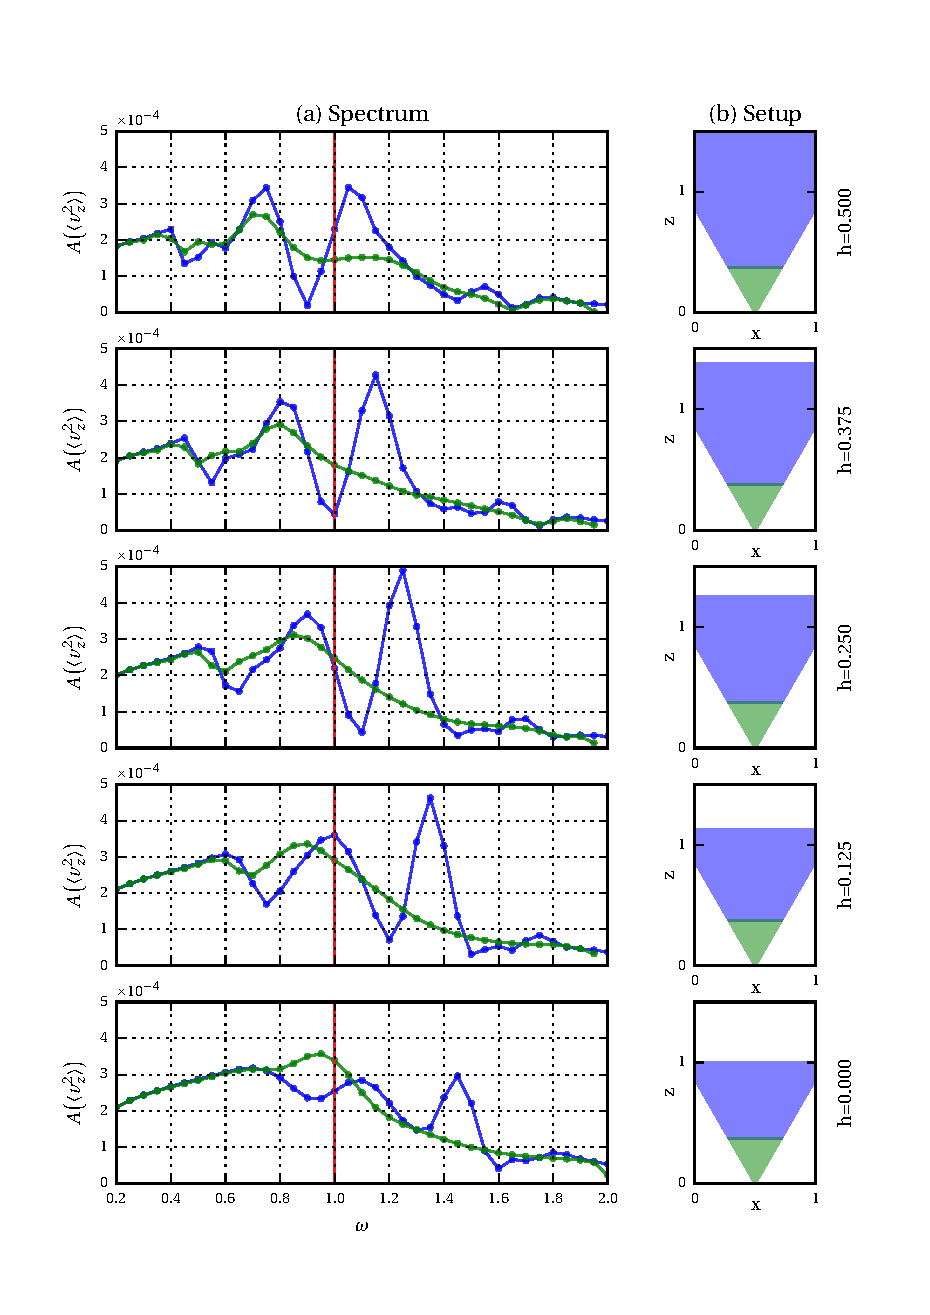
\includegraphics{gfx/cone/final/transition.pdf}
  \caption{\label{fig:cone:finaltransition}
    Simulation of Discussion}
\end{figure}


-description\\
-verfahren und serie\\
-diskussion oberer rand\\
-eigenschaften und influence oberer rand \\


Finally
-nun cone mit und ohne spitze
-teste den einfluss der oberen kante blablabla
-serien vergleich diskussion\
-helizität diskussion\\

In order to test
As a first test

\subsection{Discussion}


\section{Summary}
freeslip besser




